We perturb matched neighbor sets while holding each fitted GraphGRU and its adjacency fixed.
Each target receives the same intervention size across selection rules and graphs, between one and ten neighbors, with a mean of 9.88.
Table~\ref{tab:metric_targeted_perturbation_naics4} reports the NAICS-4 results over all matched target events.
The disconnected-node control gives zero forecast change in every graph, seed, and evaluation month.

\begin{table}[!htbp]
\centering
\begingroup
\singlespacing
\fontsize{9pt}{10.5pt}\selectfont
\setlength{\tabcolsep}{4pt}
\renewcommand{\arraystretch}{1.08}
\caption{Matched neighbor interventions under NAICS-4 at $T=14$, $H=7$, averaged over five seeds. Every rule intervenes on the same number of neighbors for each target. Removed false activations and lost positive activations are percentages of their originally activated zero-visit and positive-visit events, respectively.}
\label{tab:metric_targeted_perturbation_naics4}
\begin{adjustbox}{max width=\linewidth}
\begin{tabular}{llrrrr}
\toprule
Period & Neighbor group & \makecell{Reduction\\per neighbor} & $\Delta\mathrm{MAE}$ & \makecell{False activations\\removed (\%)} & \makecell{Positive activations\\lost (\%)} \\
\midrule
December & Training-active & $0.0026\pm 0.0003$ & $-0.016\pm 0.002$ & $40.1\pm 7.8$ & $22.5\pm 4.0$ \\
 & Recent-active & $0.0025\pm 0.0003$ & $-0.016\pm 0.002$ & $39.7\pm 7.8$ & $22.1\pm 4.2$ \\
 & Correlated & $0.0013\pm 0.0001$ & $-0.006\pm 0.001$ & $17.8\pm 3.5$ & $9.4\pm 1.4$ \\
 & Random & $0.0013\pm 0.0001$ & $-0.006\pm 0.001$ & $17.9\pm 3.5$ & $8.9\pm 1.1$ \\
 & Matched replacement & $0.0006\pm 0.0001$ & $-0.003\pm 0.001$ & $17.1\pm 2.0$ & $9.5\pm 0.8$ \\
\addlinespace[3pt]
January & Training-active & $0.0030\pm 0.0003$ & $-0.016\pm 0.001$ & $32.5\pm 5.6$ & $10.7\pm 1.1$ \\
 & Recent-active & $0.0029\pm 0.0003$ & $-0.016\pm 0.002$ & $32.3\pm 5.7$ & $10.5\pm 1.1$ \\
 & Correlated & $0.0014\pm 0.0001$ & $-0.005\pm 0.001$ & $15.2\pm 2.5$ & $4.7\pm 0.6$ \\
 & Random & $0.0014\pm 0.0001$ & $-0.006\pm 0.000$ & $14.9\pm 2.3$ & $4.4\pm 0.5$ \\
 & Matched replacement & $0.0008\pm 0.0001$ & $-0.004\pm 0.000$ & $16.3\pm 1.6$ & $5.5\pm 0.2$ \\
\bottomrule
\end{tabular}
\end{adjustbox}
\endgroup
\end{table}


Zeroing neighbors with the highest training activity reduces December MAE by \(0.016\) visits, compared with \(0.006\) for random neighbors of the same size.
Its paired joint temporal--spatial 95\% interval is \([-0.023,-0.010]\) visits.
Recent-active neighbors produce a similar reduction, while correlation-based selection is close to random selection.
The ordering persists in January, when the MAE reductions are \(0.016\) for training-active neighbors and \(0.006\) for random neighbors.
Replacing active-neighbor histories with activity-matched external histories produces smaller reductions of \(0.003\) and \(0.004\) visits in the two months.
Thus, the effect of setting histories to zero partly reflects the amount of activity removed; it exceeds the effect of replacing histories with comparable training activity.

\begin{figure}[!htbp]
\centering
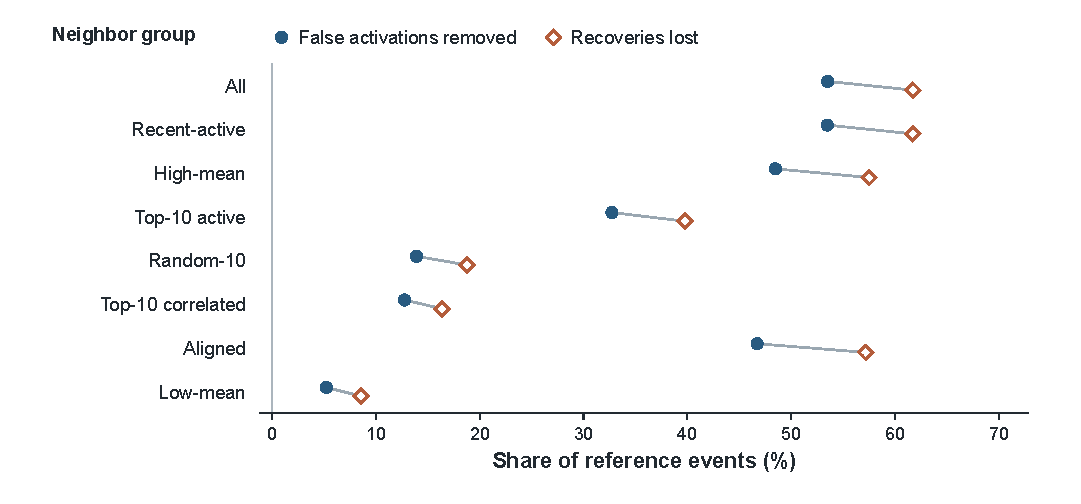
\includegraphics[scale=0.80]{art/neighbor_perturbation_tradeoff.pdf}
\caption{Matched neighbor interventions under NAICS-4 at \(T=14\), \(H=7\). Points and bars show five-seed means and standard deviations. Each percentage uses its own originally activated zero-visit or positive-visit events as the denominator.}
\label{fig:neighbor_perturbation_tradeoff}
\end{figure}

The reduction in aggregate error comes with lost positive-event detections.
In December, zeroing training-active neighbors removes \(40.1\%\) of original false activations and \(22.5\%\) of original positive activations; in January, the corresponding fractions are \(32.5\%\) and \(10.7\%\).
Recent-active selection has nearly the same tradeoff, as Figure~\ref{fig:neighbor_perturbation_tradeoff} shows.
The activity-matched replacement removes \(17.1\%\) of false activations and \(9.5\%\) of positive activations in December.
Active neighbors therefore support both correct detections and false activations, and lower aggregate MAE after their removal does not imply better detection of intermittent visits.
